\documentclass{exercices}
\usepackage{ae, aeguill, graphicx}
\usepackage{fullpage}
\usepackage{xspace}
\usepackage{color}
\usepackage{amsmath, amssymb}
\usepackage{latexsym}
\usepackage{url}
\usepackage{tikz}
\usetikzlibrary{arrows,shapes,trees,fit,decorations.pathmorphing,backgrounds}

\usepackage{verbatim}

\begin{document}

\sujet{Java lab 2 - 20 \& 21 october 2008}

The answers to the exercices below are due before \emph{22 October 2008}. 
The procedure to send the exercices is:
\begin{enumerate}
  \item Create a directory named \verb!yourname-lab2!.
  \item Copy all the \verb!.java! source files to this directory.
  \item Issue following command in a shell : \verb!gtar czvf yourname-lab2.tar.gz yourname-lab2/!
        to create a tarball.
  \item Send this tarball to \verb!pablo@sifflez.org! with subject \verb!yourname-lab2!.
\end{enumerate}

\section{Goal}
This lab is divided in two sections:
\begin{itemize}
\item
In the first section you will write a java program that keeps a list of students and teachers, sorts
this persons' list by name and prints it.
\item
In the second section you will add to this program the possibility to keep track of courses, each course
will have a teacher and many students. You will add a class that tries to find a schedule so that
no teacher has to teach two courses the same day, and no student has to follow two courses the same day.
\end{itemize}

\section{People database}
\subsection{Classes hierarchy}
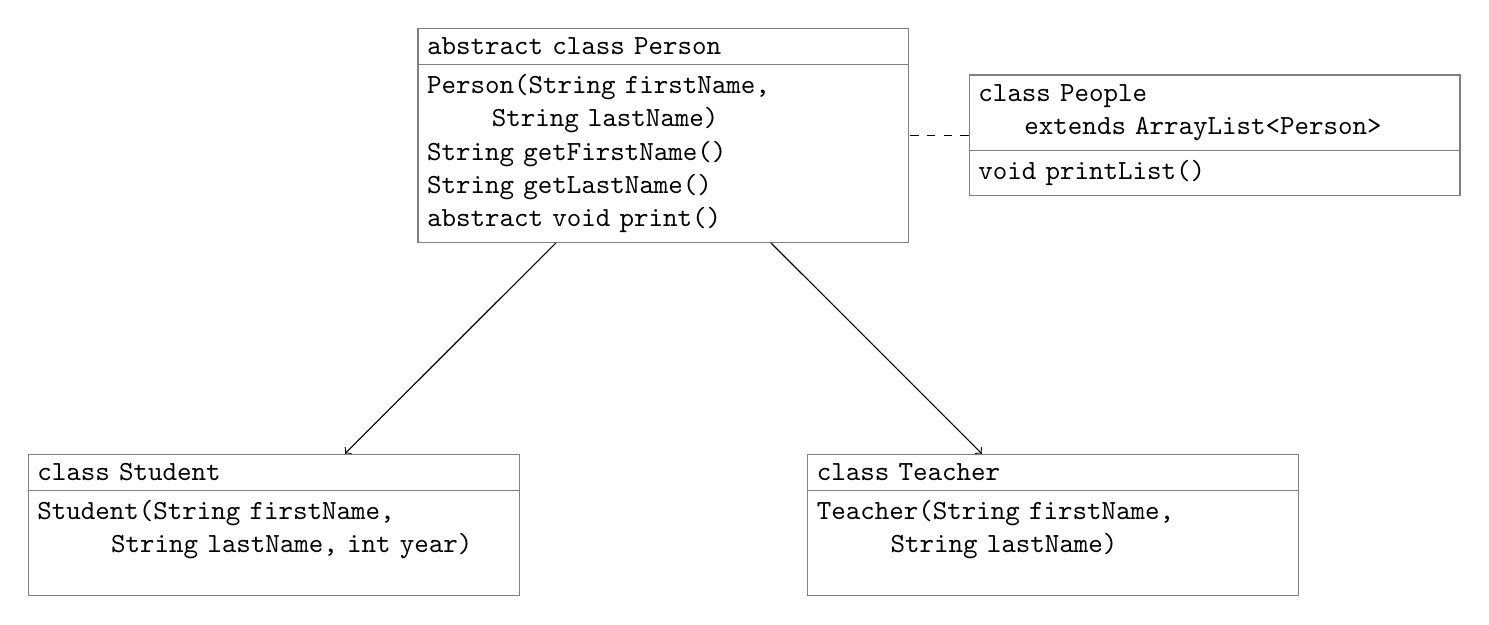
\begin{tikzpicture}
[classbox/.style={rectangle, draw=black!50, rectangle split,
  rectangle split parts=2, node distance=7cm, text width=6cm}]
  \node[classbox](Person)  {\verb!abstract class Person!\nodepart{second}
    \verb!Person(String firstName,!\newline
    \verb!       String lastName)!\newline
    \verb!String getFirstName()!\newline
    \verb!String getLastName()!\newline
    \verb!abstract void print()!
  };
\node[right of=Person,classbox](People)  {\verb!class People!\newline\verb!     extends ArrayList<Person>!\nodepart{second}
    \verb!void printList()!
  } edge[dashed] (Person);
\node[below left of=Person,classbox] (Student) {\verb!class Student!\nodepart{second}
  \verb!Student(String firstName,!\newline
  \verb!        String lastName, int year)! \newline
  } edge[<-] (Person);
\node[below right of=Person,classbox] (Teacher) {\verb!class Teacher!\nodepart{second}
  \verb!Teacher(String firstName,!\newline
  \verb!        String lastName)! \newline
  } edge[<-] (Person);
\end{tikzpicture}

\begin{exercice}[\textbf{class Person}]\\
Write an abstract class Person that implements above methods.
To store the first and last name use two private instance String variables.
\end{exercice}

\begin{exercice}[\textbf{classes Teacher and Student}]\\
Write Teacher and Student classes that extend Person.
Students should have in addition to a first and last name, a field for their current year in school. 
Teacher and Student class should implement method print which prints the person name, the person type (teacher or student) 
and in the case of students their current year.
\end{exercice}

\begin{exercice}[\textbf{class People}]\\
Write a class People that extends java.util.ArrayList<Person> class.
This class will keep the list of students and teachers.
It will provide a method printList, which calls print() for each Person it contains.
Add a main method to this class that adds some teachers and students to People, and call printList.
\end{exercice}

\subsection{Sorting persons}
Now we want to sort the persons in People, so that we can print them in alphabetical order.
To achieve this we will use method java.util.Collections.sort() and interface java.util.Comparable.
Read the documentation for interface Comparable at
\url{http://java.sun.com/j2se/1.4.2/docs/api/java/lang/Comparable.html}
and for method sort at
\url{http://java.sun.com/j2se/1.4.2/docs/api/java/util/Collections.html#sort(java.util.List)}.

\begin{exercice}[\textbf{interface Comparable<Person>}]\\
We want to specify a total order for objects of type Person. 
To do this we will modify class Person so that it implements Comparable<Person>.
We want to order persons using lexicographical order by their last name and if they have 
the same last name by their first name.

For example this would be a valid ordering:
\begin{verbatim}
  first   last

  Zoe     Amele
  Clement Dupont
  Cloe    Dupont
  Eric    Ziegler
\end{verbatim}
\end{exercice}
\begin{exercice}[\textbf{Sort People}]\\
Add a method sort to class people that sorts its Persons, using static method java.util.Collections.sort();
Test your implementation by calling printList.
\end{exercice}
\section{Courses scheduler}
\begin{tikzpicture}
[classbox/.style={rectangle, draw=black!50, rectangle split,
  rectangle split parts=2, node distance=7cm, text width=7cm}]

  \node[classbox](Course)  {\verb!class Course!\newline
\verb!     extends ArrayList<Students>!
\nodepart{second}
    \verb!Course(String name,!\newline
    \verb!       Teacher teacher)!\newline
    \verb!int getDay()!\newline
    \verb!void setDay(int dayOfWeek)!\newline
    \verb!void unschedule()!\newline
    \verb!boolean scheduled()!\newline
    \verb!Teacher getTeacher()!\newline
    \verb!boolean compatible(Course other)!\newline
  };
\node[below of=Person,classbox] (Schedule) {\verb!class Schedule!\newline
\verb!     extends ArrayList<Course>!
\nodepart{second}
  \verb!static int daysInSchoolWeek = 5!\newline
  \verb!void print()!\newline
  \verb!void checkSchedule(Course course)!\newline
  \verb!     throws IncompatibleSchedule!\newline
  \verb!void updateSchedule()!\newline
  \verb!     throws IncompatibleSchedule,!\newline
  \verb!            FoundSchedule!
  } edge[dashed] (Course);
\end{tikzpicture}

\subsection{Courses}

\begin{exercice}[\textbf{Class Course}]\\
  Create a class course with the members listed above.
  Each Course has a single teacher (provided in the constructor) and many students (added with method
  add inherited from ArrayList).
  \begin{itemize}
  \item
  Each course is either \emph{not scheduled} or \emph{scheduled for a specific day of the week, represented by an int}.
  \item
  Method setDay, allows to schedule a Course for a specific day.
  \item
  Method unschedule, set the Course to \emph{not scheduled}.
  \item
  Method scheduled, returns true if the course is scheduled.
  \item
  Method compatible, check if current course is compatible with another course. ie, they have different teachers and they have no students in common.
  \end{itemize}
\end{exercice}

\subsection{Scheduler}
Finally we are going to write a class Schedule that tries to find a compatible schedule for a list of courses.

\begin{exercice}[\textbf{Exceptions}]\\
Create two new exception classes called IncompatibleSchedule and FoundSchedule.
\end{exercice}


\begin{exercice}[\textbf{Schedule}]\\
Write a class Schedule like above but only implement method print().
The method print should print all the Courses in Schedule, and the day they are
scheduled or \verb!not scheduled! if they are not scheduled.
Add a list of courses to a Schedule and call print(), all the courses should be marked
as \verb!not scheduled!.
\end{exercice}

\begin{exercice}[\textbf{checkSchedule}]\\
Implement method checkSchedule.
This method takes a Course:
\begin{itemize}
\item if all the others courses scheduled the same day are compatible, it does nothing.
\item if one of them is not compatible, it throws exception IncompatibleSchedule.
\end{itemize}
\end{exercice}

\begin{exercice}[\textbf{updateSchedule}]\\
Implement method updateSchedule, using method checkSchedule.
This method tries to find a schedule for all the Courses, if this schedule is found it throws
ScheduleFound, if no compatible schedule exists it throws IncompatibleSchedule.

\begin{itemize}
\item To implement this method you will use a backtracking algorithm. 
\begin{enumerate}
  \item If all the courses are scheduled, throw ScheduleFound.
  \item If there still are unscheduled courses, take one of them.
  \item For each of the available days:
  \begin{enumerate}
    \item Try to schedule if for day d.
    \item call updateSchedule() recursively to try to schedule the other courses.
    \item if there is a schedule incompatibility, try another day.
  \end{enumerate}
  \item if there is no possible day on which to schedule the course, throw IncompatibleSchedule. 
\end{enumerate}
\end{itemize}
\end{exercice}
\begin{exercice}[\textbf{Test}]\\
Add some students, teachers and courses and test the scheduling algorithme. 
To avoid adding a lot of courses, you can set daysInSchoolWeek to a small value.
\end{exercice}
\end{document}
